\documentclass[10pt,twoside]{article}
\usepackage{tikz}
\usetikzlibrary{shapes,arrows.meta}
\begin{document}
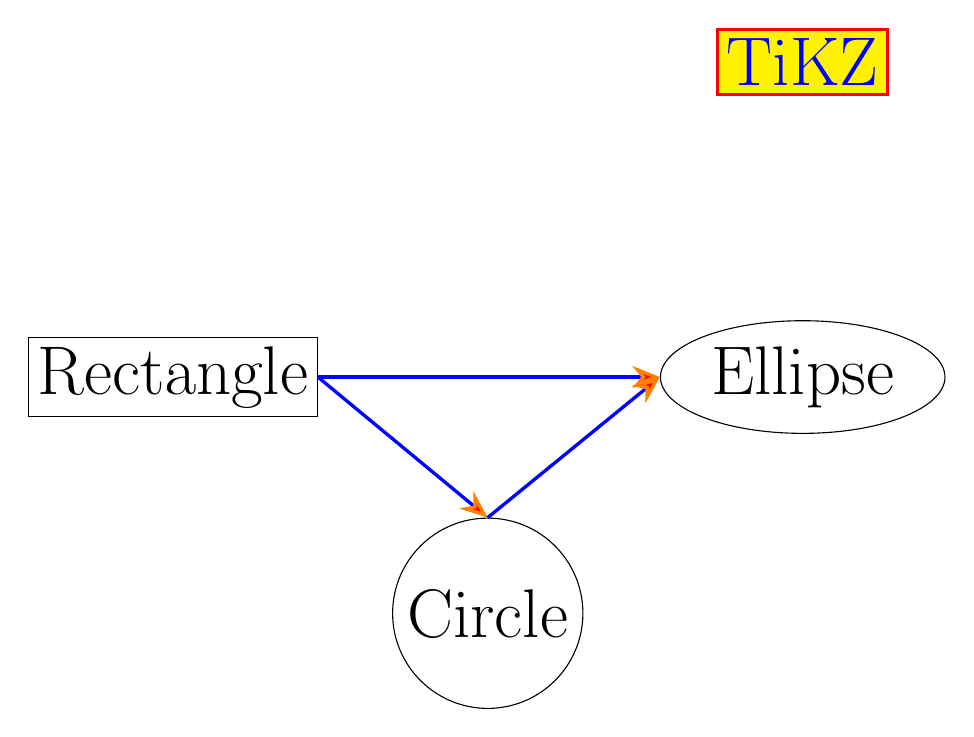
\begin{tikzpicture}
    \tikzset{my arrow/.style={blue, very thick},> = {Stealth[color=orange, fill=red,width=8pt, length=10pt]}}
    \node[draw,color=red,fill=yellow,text=blue, very thick] at (4,2)  {\Huge{TiKZ}};
    \node (r) at (-4,-2) [draw,rectangle] {\Huge{Rectangle}};
    \node (e) at (4,-2) [draw, ellipse] {\Huge{Ellipse}};
    \node (c) at (0,-5) [draw,circle] {\Huge{Circle}};

    \draw[my arrow, ->] (r.east) -- (c.north);
    \draw[my arrow, ->] (c.north) -- (e.west);
    \draw[my arrow, ->] (r.east) -- (e.west);
\end{tikzpicture}
\end{document}

